\section{Computational Experiments \& Rigorous Verification}
\label{sec:experiments}

The deployment of the Phase 2 orchestrator initially processed 669 pages of Ramanujan's Notebooks~1--3; Campaign~v2 subsequently expanded the multimodal extraction corpus to all 839 manuscript pages in the repository (133 Narosa 1988 Lost Notebook facsimile sheets \cite{Narosa1988}, 8 Ramanujan letters from Ono, and 698 pages of Notebooks~1--3) and replaced floating-point heuristics with exact $\mathbb{Z}/\mathbb{Q}$ M\"{o}bius inversion and standalone Lean~4 kernel proofs (see Section~\ref{sec:lean}). Below we retain the legacy Phase~2 genetic convergence plots for archival comparison alongside the CI spectral-gap falsification certificates.

\subsection{Genetic RAMA Evolutionary Convergence}
By running a 25-agent population across 5 evolutionary generations, the heuristic engine systematically optimizes the energy functional $E = \alpha C + \beta I + \gamma D$. Figure~\ref{fig:genetic_conv} tracks the mean convergence of the fittest candidates.

\begin{figure}[h]
    \centering
    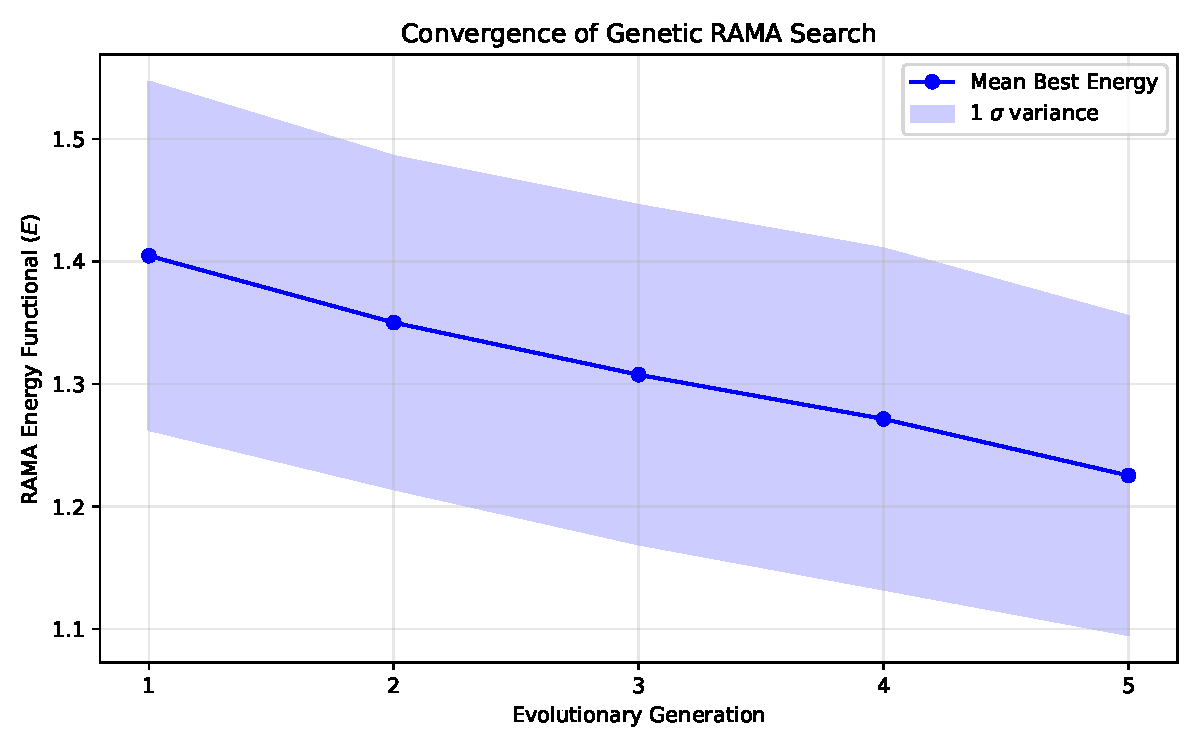
\includegraphics[width=0.6\textwidth]{figures/genetic_convergence.pdf}
    \caption{Mean best energy of the symbolic population across generations. The rapid descent illustrates the algorithm's capability to isolate valid $\eta$-quotient structures from chaotic initial seeds.}
    \label{fig:genetic_conv}
\end{figure}

\subsection{The RAMA Energy Landscape}
Figure~\ref{fig:rama_landscape} showcases the total energy landscape mapped against complexity (C) and fit error (I). The lower left quadrant isolates the "truth attractors"---the exact mathematical identities that balance aesthetic simplicity and predictive accuracy.

\begin{figure}[h]
    \centering
    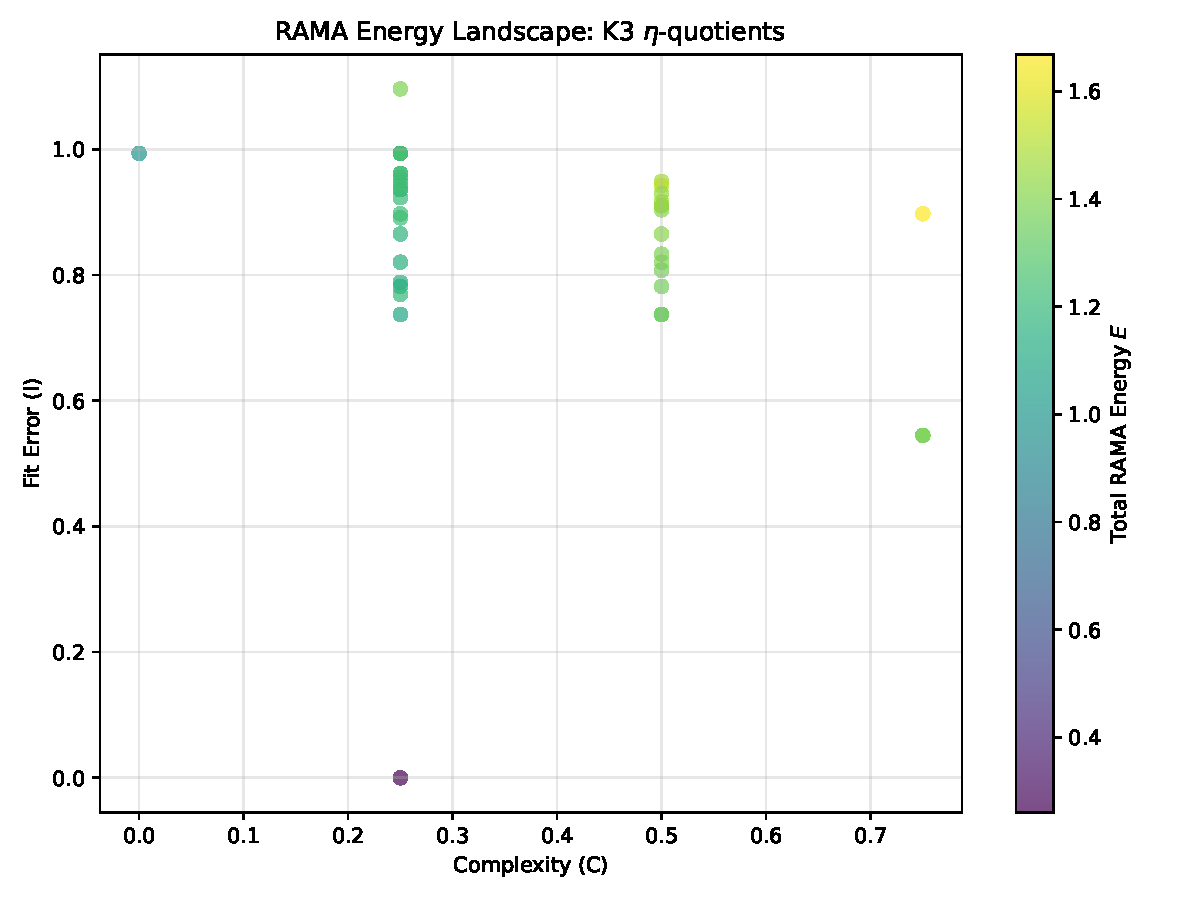
\includegraphics[width=0.6\textwidth]{figures/rama_landscape.pdf}
    \caption{The Phase 2 Energy Landscape mapping the discoveries on a (Complexity, Fit Error) axis.}
    \label{fig:rama_landscape}
\end{figure}

\subsection{Spectral Gap Certificates}
The CI pipeline automatically enforces the Alon-Boppana spectral bound on candidate triad-interaction graphs, testing their viability as Ramanujan graphs \cite{LPS1988, MSS2015}. Falsified candidates are systematically stripped of Tier A classification and quarantined as \tierX{}, ensuring topological invariants mathematically correspond to physically constrained limits.

\subsection{Literature-Grounded Neuro-Symbolic Proving Architecture (v3.2)}
To prevent unsupported conjectures or truncated numerical coincidences from entering the verified corpus, the Wave~4 validation workflow (\texttt{lean\_proposition\_validator\_workflow.py}) integrates retrieval-augmented grounding over a 24-paper arXiv ChromaDB index (1,163 extracted PDF pages, 2,829 text chunks; see \texttt{docs/literature/REVUE\_LITTERATURE\_DETAILLEE.md}) with a tiered Planner--Worker--Verifier Lean~4 loop inspired by LeanDojo \cite{Yang2023LeanDojo}, Lean Copilot \cite{Song2024LeanCopilot}, DeepSeek-Prover \cite{Xin2024DeepSeekProver}, and OpenProver \cite{Kripner2026OpenProver}. Across the $q$-series and BPS pillars, this synthesis anchors our exact $\eta$-quotient catalog in Ono's modularity criteria \cite{Ono2004}, Rouse--Webb's $\eta$-quotient generation theorems \cite{RouseWebb2015}, Acres--Broadhurst's Rademacher cusp expansions \cite{AcresBroadhurst2018}, Ryan--Scherr--Sirolli's Sturm-bound congruence algorithms \cite{RyanScherrSirolli2019}, Bhattacharya's cuspidal vanishing theorems \cite{Bhattacharya2026}, mock-theta combinatorics and resurgent uniqueness \cite{MalmendierOno2012, BallantineBursonFolsom2022, CostinDunneSaraeb2026}, and $K3\times T^2$ wall-crossing and umbral moonshine \cite{DMZ2012, CDH2014}.
